%%%%%%%%%%%%%%%%%%%%%%%%%%%%%%%%%%%%%%%%%
% Arsclassica Article
% LaTeX Template
% Version 1.1 (1/8/17)
%
% This template has been downloaded from:
% http://www.LaTeXTemplates.com
%
% Original author:
% Lorenzo Pantieri (http://www.lorenzopantieri.net) with extensive modifications by:
% Vel (vel@latextemplates.com)
%
% License:
% CC BY-NC-SA 3.0 (http://creativecommons.org/licenses/by-nc-sa/3.0/)
%
%%%%%%%%%%%%%%%%%%%%%%%%%%%%%%%%%%%%%%%%%

%----------------------------------------------------------------------------------------
%	PACKAGES AND OTHER DOCUMENT CONFIGURATIONS
%----------------------------------------------------------------------------------------

\documentclass[
10pt, % Main document font size
a4paper, % Paper type, use 'letterpaper' for US Letter paper
oneside, % One page layout (no page indentation)
%twoside, % Two page layout (page indentation for binding and different headers)
headinclude,footinclude, % Extra spacing for the header and footer
BCOR5mm, % Binding correction
]{scrartcl}

%%%%%%%%%%%%%%%%%%%%%%%%%%%%%%%%%%%%%%%%%
% Arsclassica Article
% Structure Specification File
%
% This file has been downloaded from:
% http://www.LaTeXTemplates.com
%
% Original author:
% Lorenzo Pantieri (http://www.lorenzopantieri.net) with extensive modifications by:
% Vel (vel@latextemplates.com)
%
% License:
% CC BY-NC-SA 3.0 (http://creativecommons.org/licenses/by-nc-sa/3.0/)
%
%%%%%%%%%%%%%%%%%%%%%%%%%%%%%%%%%%%%%%%%%

%----------------------------------------------------------------------------------------
%	REQUIRED PACKAGES
%----------------------------------------------------------------------------------------

\usepackage[
nochapters, % Turn off chapters since this is an article        
beramono, % Use the Bera Mono font for monospaced text (\texttt)
eulermath,% Use the Euler font for mathematics
pdfspacing, % Makes use of pdftex’ letter spacing capabilities via the microtype package
dottedtoc % Dotted lines leading to the page numbers in the table of contents
]{classicthesis} % The layout is based on the Classic Thesis style

\usepackage{arsclassica} % Modifies the Classic Thesis package

\usepackage[T1]{fontenc} % Use 8-bit encoding that has 256 glyphs

\usepackage[utf8]{inputenc} % Required for including letters with accents

\usepackage{graphicx} % Required for including images
\graphicspath{{Figures/}} % Set the default folder for images

\usepackage{enumitem} % Required for manipulating the whitespace between and within lists

\usepackage{lipsum} % Used for inserting dummy 'Lorem ipsum' text into the template

% \usepackage{subfig} % Required for creating figures with multiple parts (subfigures)

\usepackage{amsmath,amssymb,amsthm} % For including math equations, theorems, symbols, etc

\usepackage{varioref} % More descriptive referencing

%----------------------------------------------------------------------------------------
%	THEOREM STYLES
%---------------------------------------------------------------------------------------

\theoremstyle{definition} % Define theorem styles here based on the definition style (used for definitions and examples)
\newtheorem{definition}{Definition}

\theoremstyle{plain} % Define theorem styles here based on the plain style (used for theorems, lemmas, propositions)
\newtheorem{theorem}{Theorem}

\theoremstyle{remark} % Define theorem styles here based on the remark style (used for remarks and notes)

%----------------------------------------------------------------------------------------
%	HYPERLINKS
%---------------------------------------------------------------------------------------

\hypersetup{
%draft, % Uncomment to remove all links (useful for printing in black and white)
colorlinks=true, breaklinks=true, bookmarks=true,bookmarksnumbered,
urlcolor=webbrown, linkcolor=RoyalBlue, citecolor=webgreen, % Link colors
pdftitle={}, % PDF title
pdfauthor={\textcopyright}, % PDF Author
pdfsubject={}, % PDF Subject
pdfkeywords={}, % PDF Keywords
pdfcreator={pdfLaTeX}, % PDF Creator
pdfproducer={LaTeX with hyperref and ClassicThesis} % PDF producer
} % Include the structure.tex file which specified the document structure and layout

\usepackage{geometry}
 \geometry{
 left=30mm,
 top=10mm,
 tmargin=15mm,
 headheight=5mm,
 bottom=15mm,
 }

% \usepackage{subfigure}
% \usepackage{caption,subcaption}
\usepackage{graphicx}
\usepackage{subcaption}
\usepackage{float}
\captionsetup{compatibility=false}

\hyphenation{Fortran hy-phen-ation} % Specify custom hyphenation points in words with dashes where you would like hyphenation to occur, or alternatively, don't put any dashes in a word to stop hyphenation altogether

%----------------------------------------------------------------------------------------
%	TITLE AND AUTHOR(S)
%----------------------------------------------------------------------------------------

\title{\normalfont{Tutorial outline}} % The article title
\date{} % An optional date to appear under the author(s)

% \titleformat{\chapter}[display]
%   {\normalfont}{\Large\scshape\chaptertitlename\ \thechapter}{0pt}{\LARGE\bfseries #1}
% \titlespacing*{\chapter}
%   {0pt}{65pt}{40pt}

%----------------------------------------------------------------------------------------

\begin{document}
\maketitle % Print the title/author/date block

\section{Detailed description}
\label{sec:draft}
This tutorial will be divided in three sections, covering three and a half hours with a 30 minutes break, as specified. 

\subsection{\textbf{Setting up a basic scenario (1 hour)}}
At the beginning of this section, a mission demo for an AUV will be detailed to the audience, together with the steps to implement it in the simulator.
The mission will consist of an AUV which has to autonomously hover over a pipeline while creating a batymetry map of the surroundings and recording with a camera to assess its state after.
Following this, the Gazebo simulator and its ROS interface will be presented while setting up the scenario and the most basic AUV system.

\begin{figure}[h]
    \centering
    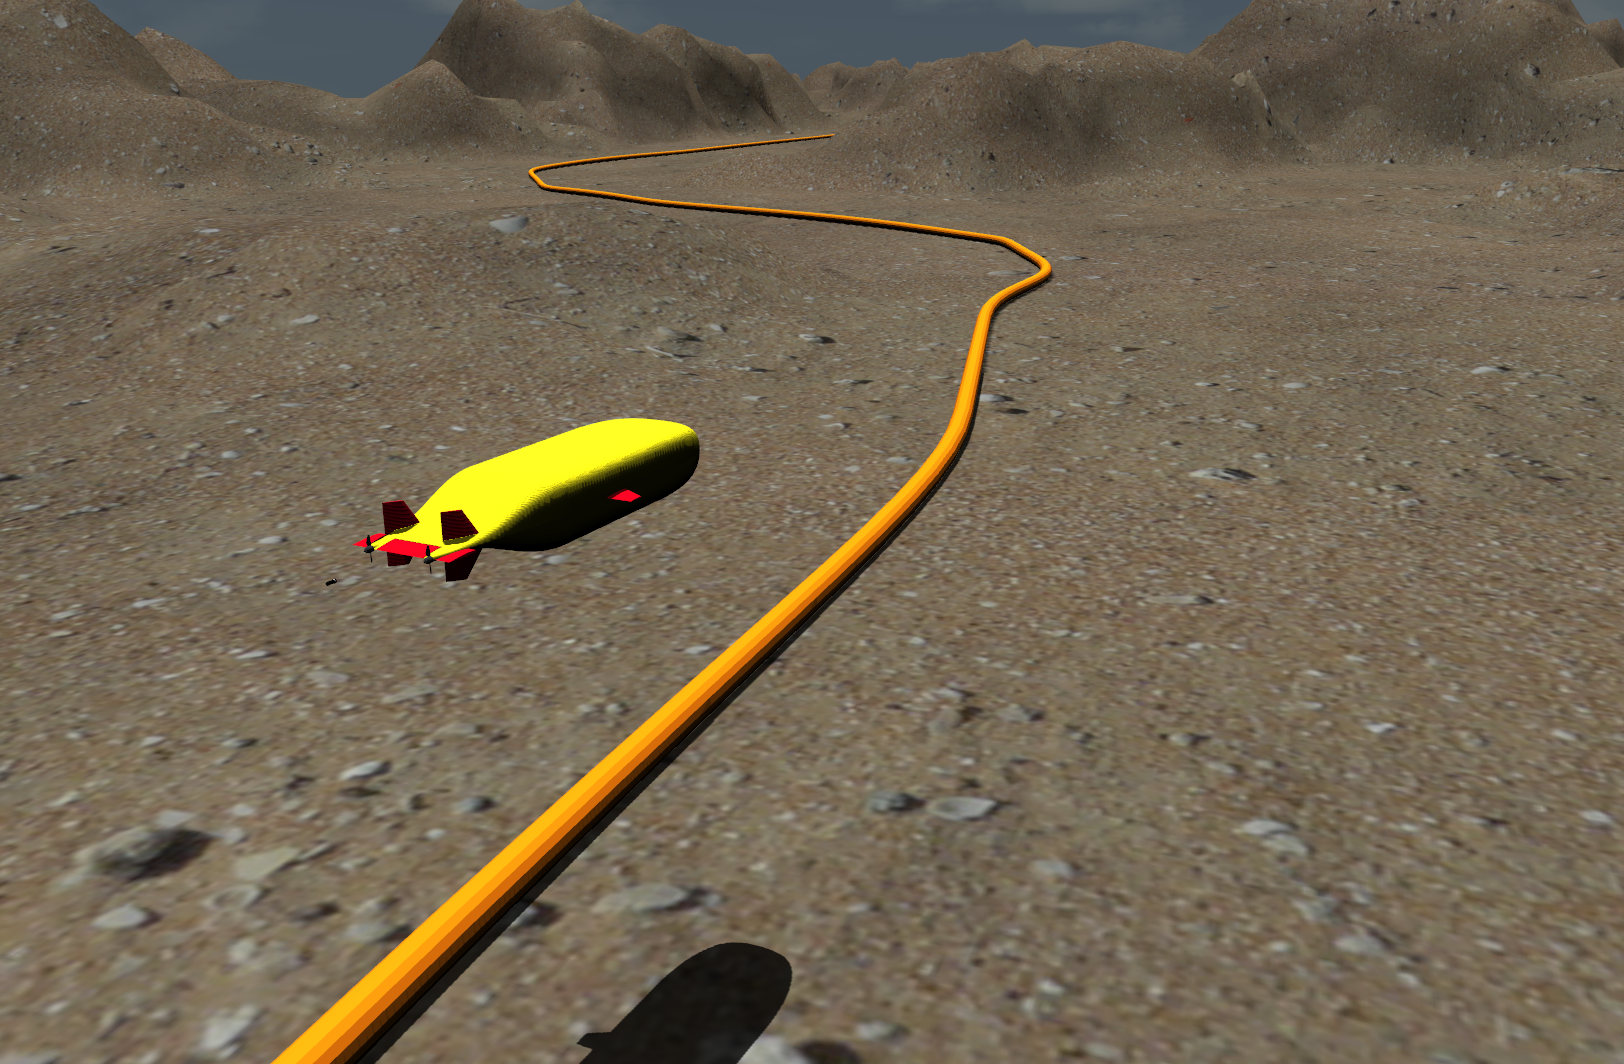
\includegraphics[width=0.9\linewidth]{Figures/sim_pipeline.png}
    \caption{Simulation of pipeline inspection mission with LoLo.}
\label{fig:lolo_gazebo}
\end{figure}

Thus, the main steps in this section are:
\begin{enumerate}
	\item Introducing the SMARC simulator, explaining the AUV mission and reasoning on the advantages of simulating before deploying a vehicle.
	\item Creating a simple subsea scenario in Gazebo consisting in a rocky seabed and a pipeline.
	\item Launching a LoLo AUV in the simulator with its most basic ROS components and a manual controller.
\end{enumerate}

A capture of the expected output of the listed tasks can be seen in \ref{fig:lolo_gazebo}.

\subsection{\textbf{Building the AUV system (1 hour)}}
In this section, the attendees will be introduced to the navigation architecture of an AUV through a hands-on setup of its basic components, already existing in the simulator.
In \ref{fig:auv_system} a high-level overview of the system to have implemented by the end of the section can be seen.
The sensors, actuators and software components will be explained, and instances of them will be plugged in the system so that the LoLo AUV can perform the autonomous inspection mission over the pipeline.

\begin{figure}[h]
    \centering
    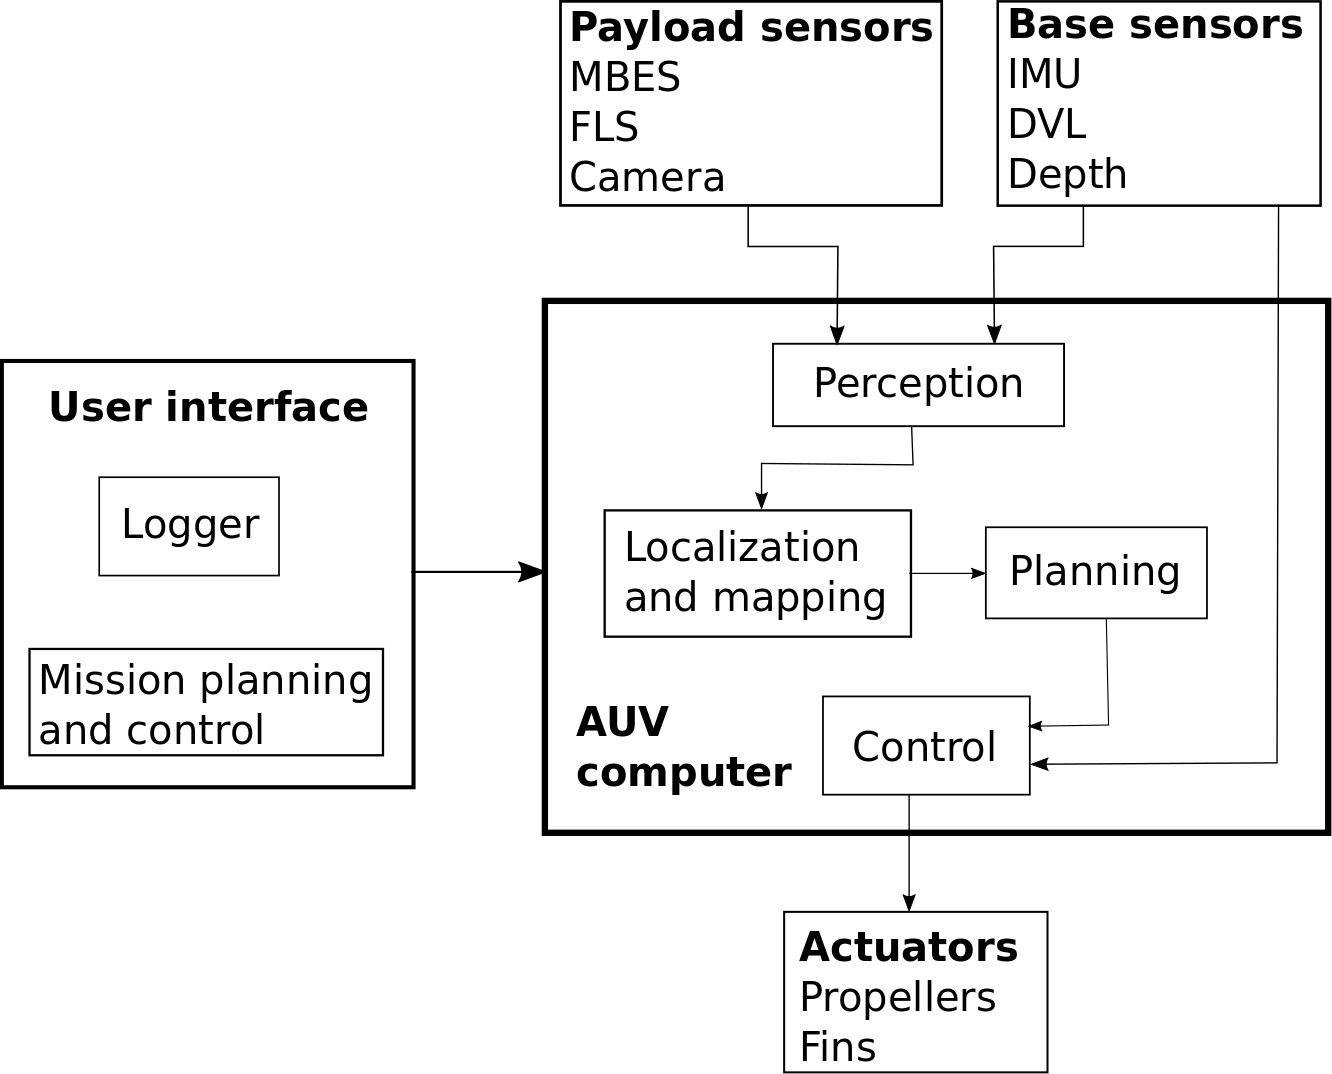
\includegraphics[width=0.9\linewidth]{Figures/auv_system.png}
    \caption{Overview of an AUV system architecture.}
\label{fig:auv_system}
\end{figure}


\subsection{\textbf{Running the demo, visualizing and logging data (1 hour)}}
The final hour will be devoted to launching the previous AUV system in the scenario created and running the final demo.
While doing so, the audience will be try the basic capabilities of the user interface during an AUV mission in the simulator in order to evaluate the current state of the mission and its final success after completion.
Attendees will put together the output from previous sections and get familiar with standard data recording, visualization and diagnosing tools in ROS such as RVIZ or rqt.

\begin{figure}[h]
    \centering
    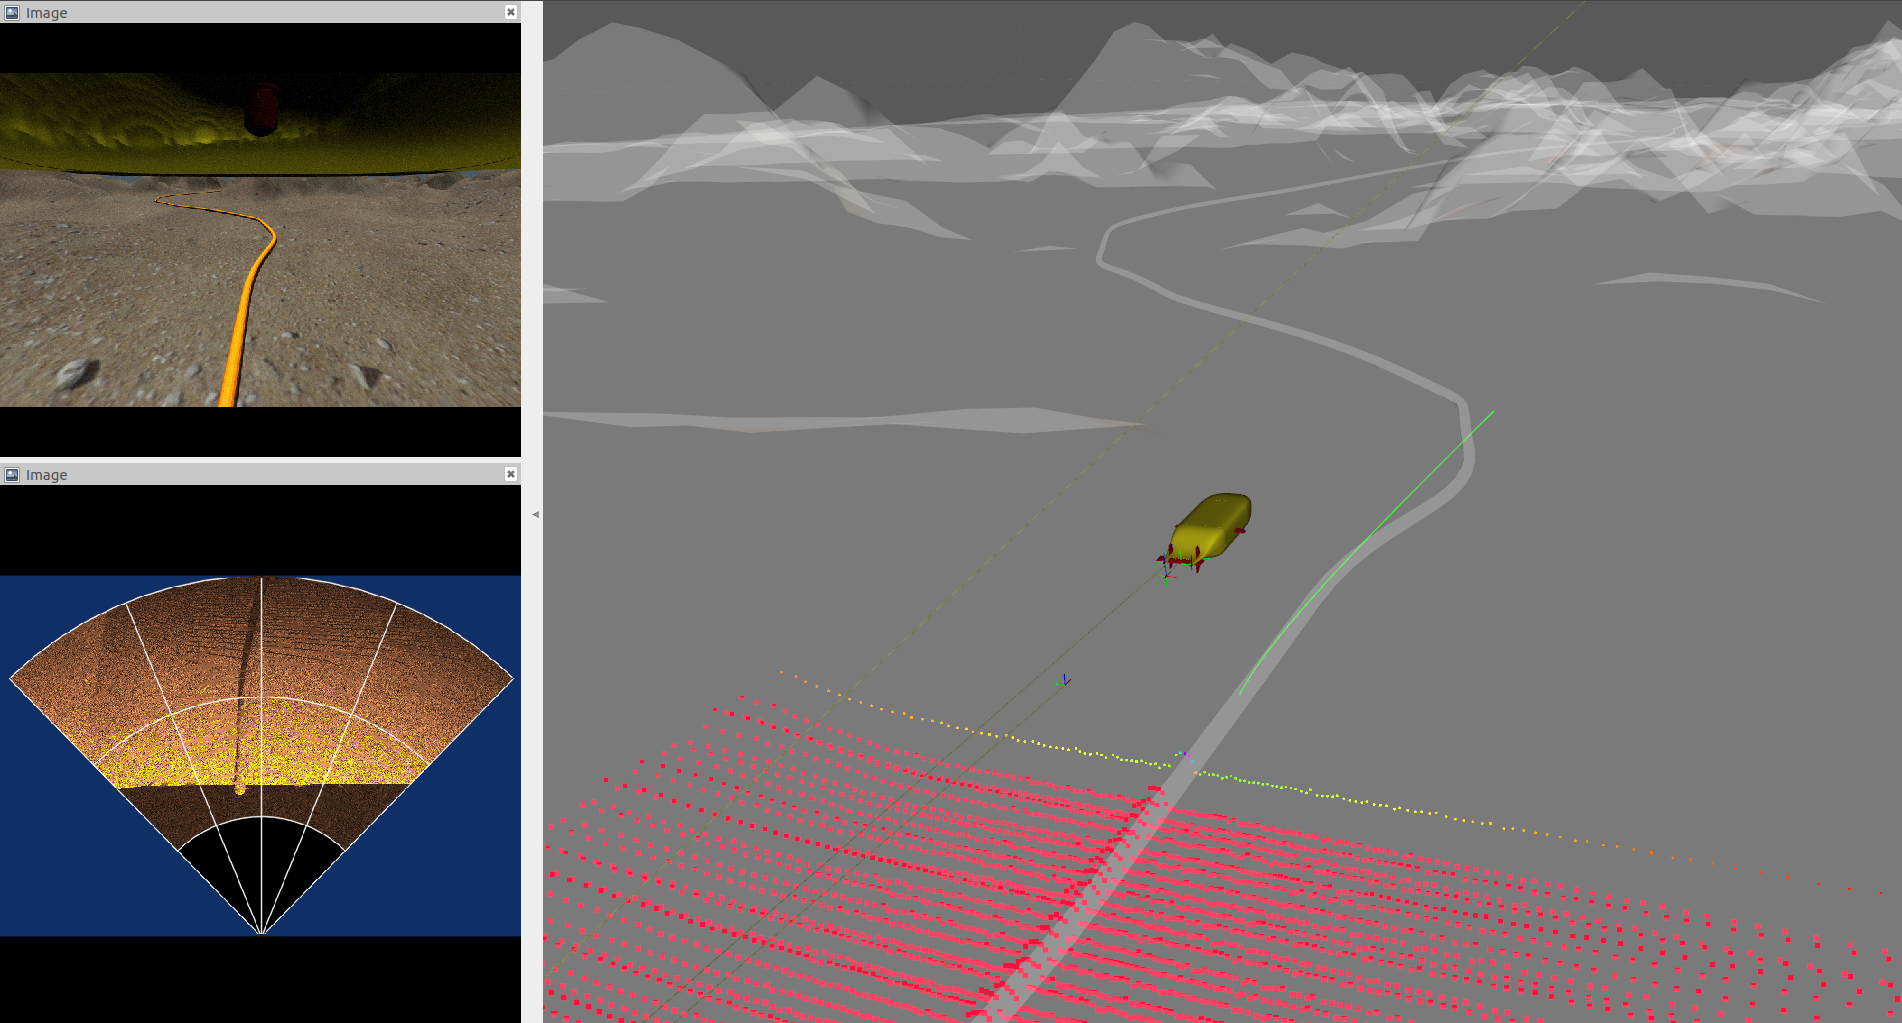
\includegraphics[width=0.9\linewidth]{Figures/rviz_pipeline.png}
    \caption{Data visualization during mission in RVIZ, including bottom camera and FLS outputs, together with the bathymetry map from the MBES in red.}
\label{fig:lolo_rviz}
\end{figure}

%----------------------------------------------------------------------------------------
\section{Description of the practical demo and exercises}
\label{sec:demo}
This tutorial is meant to be a mainly hands-on session in which the audience will follow the instructions from the main presenter to implement the proposed demo.
The different steps in each session described above are designed to be very modular, allowing each of them to be checked separately and put together as a final step.
In order to respect the timing of the session, the solutions will be provided at the end of each step, so that every attendee can keep up and have a running system by the end of the sections.
\\

\subsection{\textbf{Presentation}}
The main presenter will carry out each step required to set up the demo in front of the audience, expecting the attendants to follow up and execute the same instructions.
At the same time, some basic concepts on the subject of the section will be explained.
The second presenter will meanwhile try to answer individual queries and help execute the tasks to those who might need it.

As an example, while presenting the control module in the AUV system in \ref{fig:auv_system}, the generalities of this components in a mobile platform will be briefly discussed, different controller instances will be mentioned and finally, a controller will be added to the system.

\subsection{\textbf{Exercises}}
There will be mainly three kinds of exercises for the audience to work on individually or in groups while following the talk:

\begin{itemize}
	\item Manipulate the simulation environment, adding components to the scenario or modifying their characteristics.
	\item Work with the launching tools used in ROS and Gazebo to bring up robots and their systems. 
	Use these tools to configure the navigation system in the AUV.
	\item Utilize standard tools such as RVIZ, ROS rqt or rosbags to visualize and record mission data as in \ref{fig:lolo_rviz}.
\end{itemize}

None of the tasks requires previous knowledge of programming or building an application.
Only high-level, XML-like language will be used to work with the AUV launch system.

\subsection{\textbf{Feedback and support}}
The attendants will be given colored sticky notes to convey feedback on the development of the session. 
One color will indicate the participant has a question or needs assistance, so that they can stick it on a visible place on their workstation and let the presenters know they need support.
The other color will show success implementing an exercise.
With this method, the presenters can quickly adjust the pace of the session to the audience.


% \begin{figure}[h]
%     \centering
%     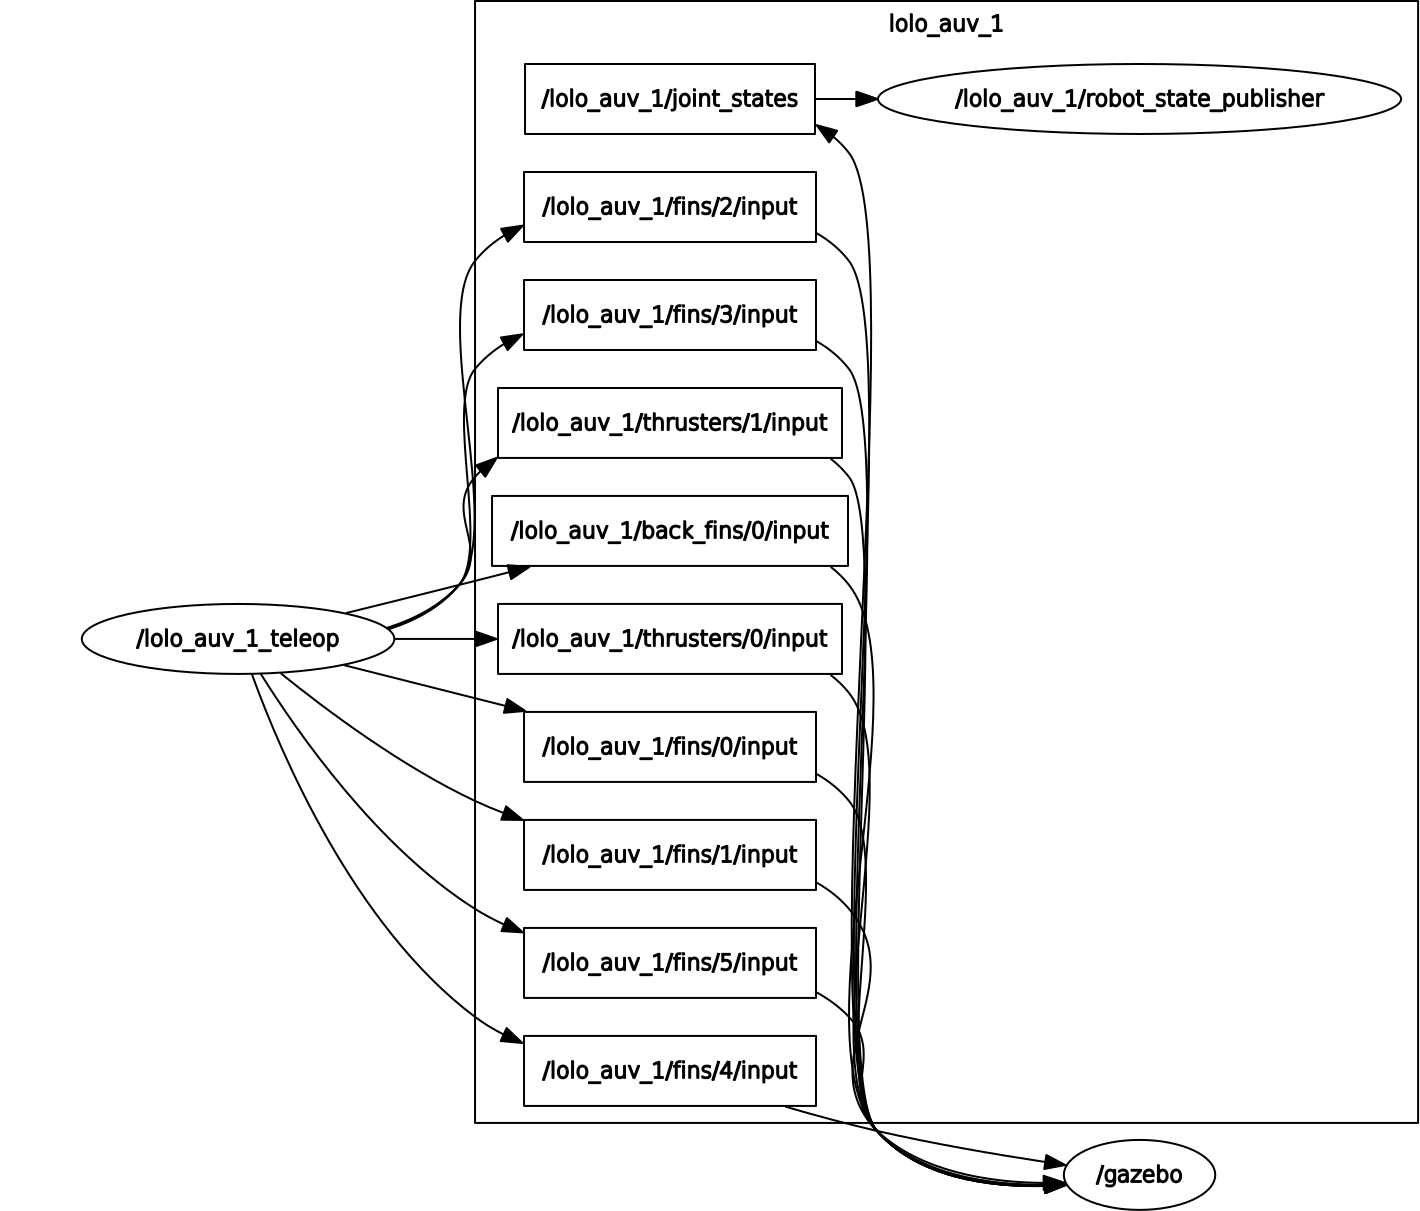
\includegraphics[width=0.9\linewidth]{Figures/rqt_graph_ex.png}
%     \caption{Data visualization during mission in RVIZ, including bottom camera and FLS outputs, together with the bathymetry map from the MBES in red.}
% \label{fig:lolo_rviz}
% \end{figure}

% \begin{figure}[h]
%     \centering
%     \begin{subfigure}[b]{0.49\textwidth}
%         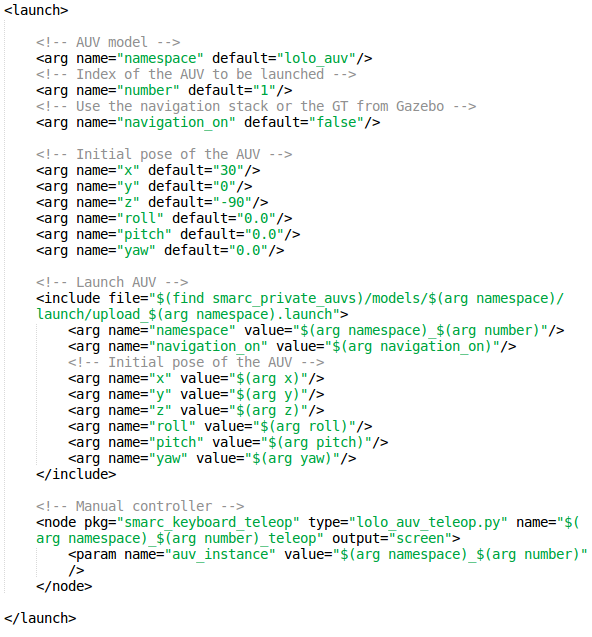
\includegraphics[width=\textwidth]{Figures/launch.png}
%     \end{subfigure}
%      %add desired spacing between images, e. g. ~, \quad, \qquad, \hfill etc. 
%       %(or a blank line to force the subfigure onto a new line)
%     \begin{subfigure}[b]{0.49\textwidth}
%         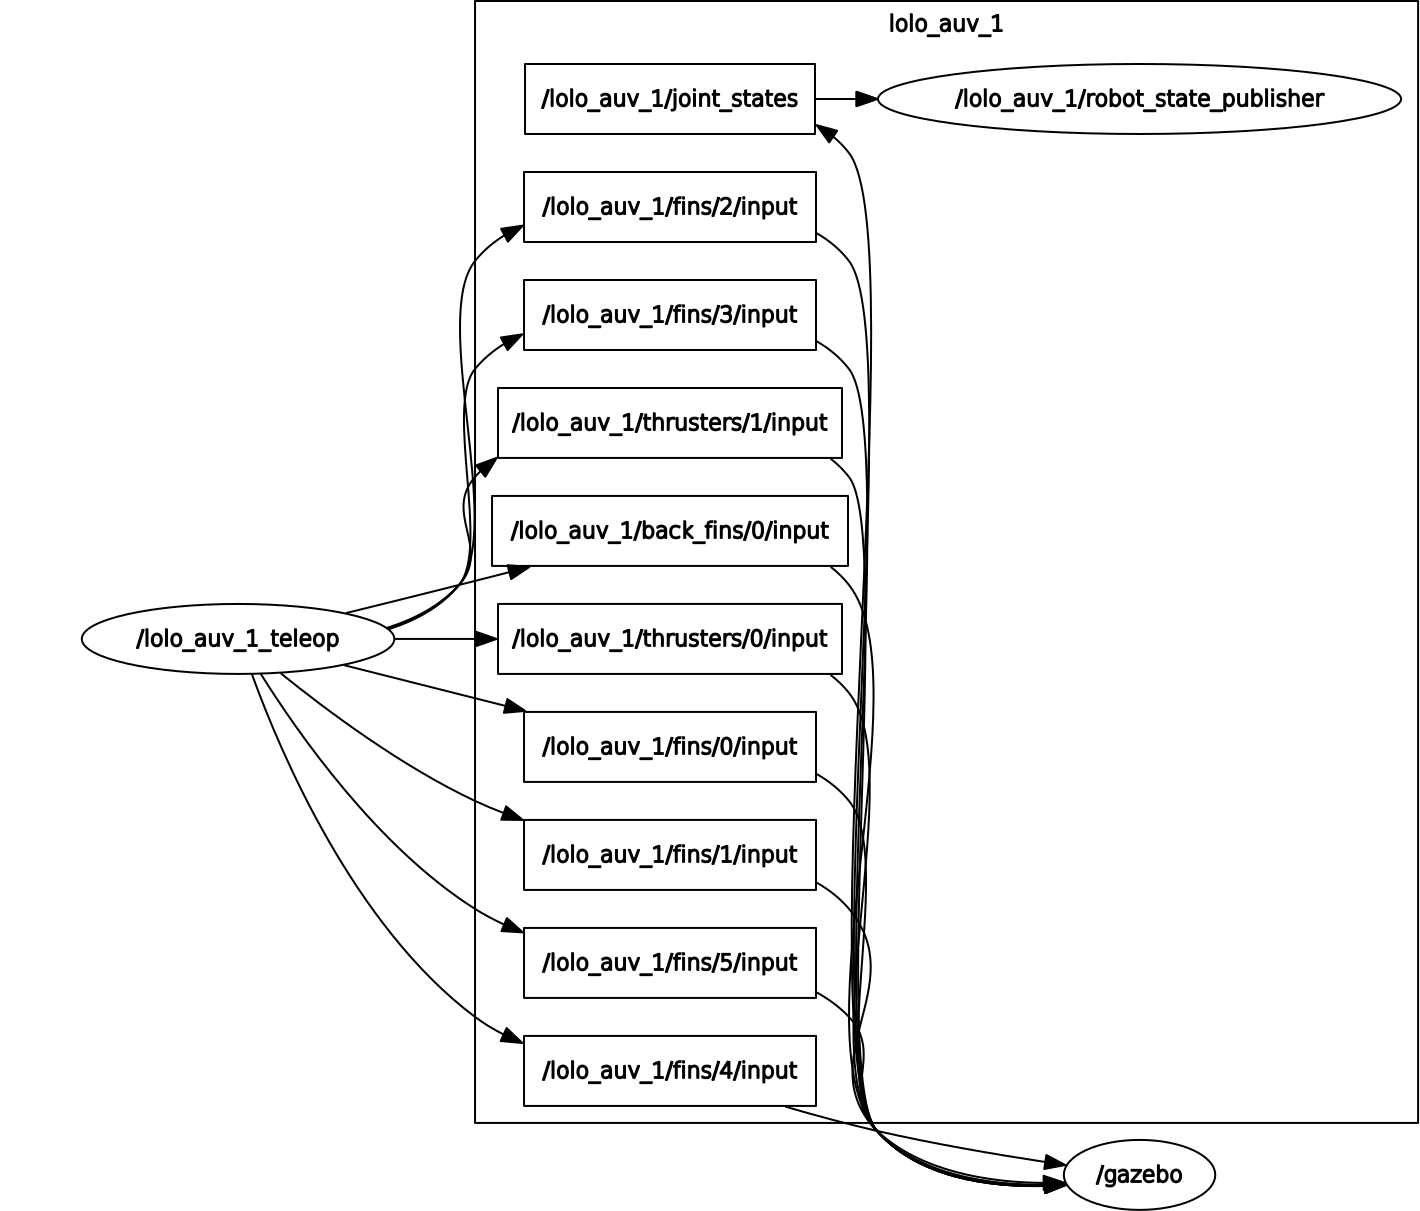
\includegraphics[width=\textwidth]{Figures/rqt_graph_ex.png}
%     \end{subfigure}
% \end{figure}

\end{document}